\documentclass[12pt,a4paper,oneside]{ctexart}
\usepackage{amsmath, amsthm, amssymb, graphicx, float}

%导言区
\title{课程《控制工程》笔记}
\author{NH5}
\date{更新于2025.3.29}

\begin{document}
\maketitle
\section{线性系统的数学描述}
通过数学模型描述线性系统.常见数学模型有:输入输出描述,状态空间描述,图形化描述

\subsection{线性系统时域数学模型——微分方程}
\subsubsection{微分方程描述}
线性定常系统的输入输出关系微分方程标准形式:
\begin{align*}
    &c^{(n)}(t) + a_1c^{(n-1)}(t) + ... + a_{n-1}c^{(1)}(t) + a_nc(t)\\
    = &b_0r^{(m)}(t) + b_1r^{(m-1)}(t) + ... + b_{m-1}r^{(1)}(t) + b_mr(t)
\end{align*}
$c(t)$是输出信号,$r(t)$是输入信号

数学模型相同的各种系统成为相似系统,在相似系统中,作用相同的变量称为相似变量.

一种系统的研究可以通过相似系统的概念推广到其他系统中,同样的,可以用一种易实现的系统代替难实现的系统.

有些方程是非线性微分方程,可以通过在平衡点用Talor级数近似的方式转化成线性方程

\subsubsection{单位脉冲响应描述}
前述方法是通过基于物理规律等的对系统的分析得到方程的方式,如分析电路.

有些情况下,我们对于系统内部结构未知,可以通过测量输入输出的得到一些数据,通过这些数据建立方程

系统是线性定常、零初始条件($t=0$时系统响应及各阶导数为$0$).则有
\[
    H:r(t) \to c(t),c(t) = H[r(t)]
\]

单位脉冲函数:
\[
    r(t)=\begin{cases}
        \frac{A}{\varepsilon}, &0<t<\varepsilon \\
        0, & t<0,t>\varepsilon
    \end{cases}
\]
当$A=1,\varepsilon \to 0$,称为单位脉冲函数$\delta(t)$

单位脉冲响应:

零初始条件下,LTI系统在$\delta(t)$作用下输出:
\[
    g(t) = H[\delta (t)]
\]

零初始条件下,LTI系统在不同输入信号作用下的输出:
\begin{align*}
    A_1\delta (t - \tau_1) + A_2\delta (t - \tau_2)&= A_1g(t - \tau_1) + A_2g(t - \tau_2)\\
    \sum_{\tau=0}^{\infty}r(\tau)\delta(t-\tau)\varepsilon &= \sum_{\tau=0}^{\infty}r(\tau)g(t-\tau)\varepsilon
\end{align*}

对于一段连续输入信号有:
\begin{align*}
    c(t) &= \int_{0}^{t}g(t-\tau)r(\tau)d\tau\\
    c(t) &= \int_{0}^{t}g(\tau)r(t-\tau)d\tau
\end{align*}

\subsection{传递函数}
\subsubsection{传递函数的定义和性质}
Laplace变换:
\[
    F(s) = L[f(t)] = \int_{0}^{\infty}f(t)e^{-st}dt
\]

设$C(s)=L[c(t)],R(s)=L[r(t)]$,且满足如下零初始条件:
\begin{align*}
    &c(0) = c^{(1)}(0) = ... = c^{(n-1)}(0) = 0\\
    &r(0) = r^{(1)}(0) = ... = r^{(m-1)}(0) = 0
\end{align*}
可得
\[
    G(s) = \frac{C(s)}{R(s)} = \frac{\sum_{0}^{m}b_ks^{m-k}}{\sum_{0}^{n}a_ks^{n-k}} = \frac{M(s)}{N(s)}
\]
$M(s),N(s)$分别被称为传递函数$G(s)$的分子多项式与分母多项式

传递函数的特征方程是$N(s)=0$,特征根是特征方程的解,
传递函数零点是$M(s)=0$的解,传递函数的极点是特征根

\subsubsection{几种典型模型}
一、比例环节/放大环节
\[
    c(t)=Kr(t),G(s)=K
\]
$K$为增益

特点:输入输出量成比例,无失真和时间延迟

实例:电子放大器,齿轮,电阻(电位器),感应式变送器等

二、惯性环节
\[
    Tc'(t) + c(t) = Kr(t),G(s) = \frac{K}{Ts+1}
\]
其中为$T$时间常数,$K$为比例系数

特点:含一个独立的储能元件,对突变的输入,其输出不能立即复现,输出无振荡

实例:直流伺服电动机的励磁回路、RC电路

三、纯微分环节
\[
    c(t)=Tr'(t),G(s)=Ts
\]

特点:输出量正比输入量变化的速度,能预示输入信号的变化趋势

实例:实际中没有纯粹的微分环节,它总是与其他环节并存的.
实际中可实现的微分环节都具有一定的惯性,其传递函数如下
\[
    G(s) = \frac{Ts}{Ts+1}
\]

四、积分环节
\[
    c(t)=K\int r(t)dt,G(s)=\frac{K}{s}
\]

特点:输出量与输入量的积分成正比例,当输入消失,
输出具有记忆功能;具有明显的滞后作用;可以改善稳态性能

实例:电动机角速度与角度间的传递函数、电容充电、模拟计算机中的积分器等

五、二阶震荡环节
\begin{align*}
    &T^2c''(t)+2\zeta Tc'(t)+c(t) = r(t),0\le \zeta <1\\
    &G(s) = \frac{\omega_n^2}{s^2+2\zeta \omega_ns+\omega_n^2},0\le \zeta <1
\end{align*}
其中$\omega_n=\frac{1}{T}$,$\zeta$称为振荡环节的阻尼比,$T$为时间常数,
为系统的自然振荡角频率(无阻尼自振角频率)

特点:环节中有两个独立的储能元件,可进行能量交换,输出有振荡

实例:RLC电路传递函数,机械弹簧阻尼系统的传递函数

六、纯时延环节
\[
    c(t)=r(t-\tau),G(s)=e^{-\tau s}
\]
$\tau$称为该环节的延迟时间

特点:输出量能准确复现输入量,但要延迟一固定的时间间隔$\tau$

实例:管道压力、流量等物理量的控制,其数学模型就包含有延迟环节

\subsection{结构图}
根据不同功能,可将系统划分为若干环节或子系统,每个子系统的功能用一个单向性的函数方块来表示

方块中填写表示这个子系统的传递函数,输入量加到方块上,那么输出量就是传递结果

根据系统中信息的传递方向,将各个子系统的函数方块用信号线顺次连接起来,就构成了系统的结构图,又称系统的方块图

如下图所示
\begin{figure}[H]
    \centering
    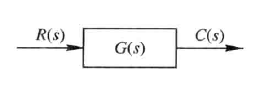
\includegraphics[width=8cm]{photos/结构图原件.png}
\end{figure}

对于闭环系统,需引入两个新符号,分别称为相加点(比较点、综合点)和分支点(引出点、测量点).
相加点是系统的比较元件,表示两个以上信号的代数运算.
箭头指向的信号流线表示它的输入信号,箭头离开它的信号流线表示它的输出信号;
附近的$+$、$-$号表示信号之间的运算关系是相加还是相减

如下图,相加点如(a),分支点如(b)
\begin{figure}[H]
    \centering
    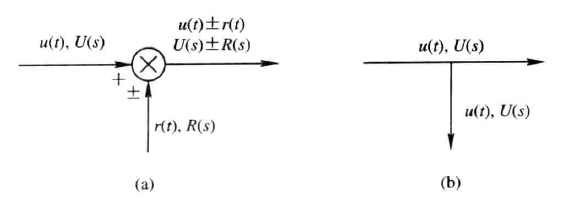
\includegraphics[width=8cm]{photos/相加点和分支点.png}
\end{figure}

\subsubsection{闭环系统结构图}
一、无扰动作用的闭环系统

基本结构如下图
\begin{figure}[H]
    \centering
    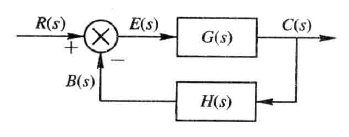
\includegraphics[width=8cm]{photos/无扰动闭环系统.png}
\end{figure}

其中$E(s)$,$B(s)$分别为偏差信号和反馈信号的Laplace变换,
$H(s)$为闭环系统中的反馈传递函数

系统中存在如下关系:
\begin{align*}
    C(s)&=G(s)E(s)\\
    E(s)&=R(s)-B(s)\\
    B(s)&=H(s)C(s)
\end{align*}

开环传递函数为反馈信号与偏差信号之比,前向传递函数为输出量和偏差信号之比

如果反馈传递函数等于1,那么开环传递函数和前向传递函数相同,称这时的闭环反馈系统为单位反馈系统

闭环传递函数为系统输出量和输入量之间的关系

易得
\[
    C(s)=\frac{G(s)}{1+G(s)H(s)}R(s)
\]

二、有扰动作用的闭环系统
如下基本结构
\begin{figure}[H]
    \centering
    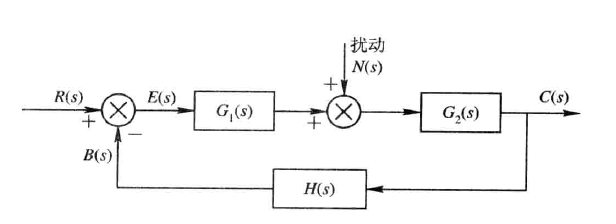
\includegraphics[width=8cm]{photos/有扰动闭环系统.png}
\end{figure}

系统对扰动$N(s)$的响应$C_N(s)$为
\[
    C_N(s)=\frac{G_2(s)}{1+G_1(s)G_2(s)H(s)}N(s)
\]

系统对参考输入量$R(s)$的响应$C_R(s)$为
\[
    C_R(s) = \frac{G_1(s)G_2(s)}{1+G_1(s)G_2(s)H(s)}R(s)
\]

参考输入量$R(s)$和扰动量$N(s)$同时作用于系统时,系统的响应$C(s)$为
\[
    C(s) = C_N(s) + C_R(s) = \frac{G_2(s)}{1+G_1(s)G_2(s)H(s)}\left[G_1(s)R(s)+N(s)\right]
\]

\subsubsection{结构图的化简}
串联的简化:传递函数相乘
\begin{figure}[H]
    \centering
    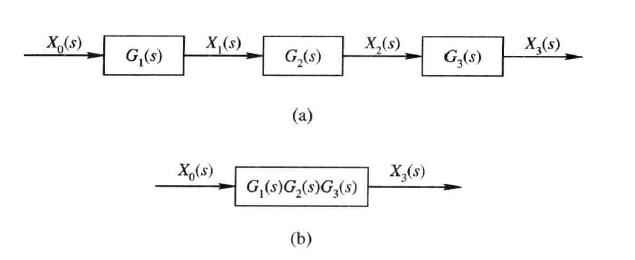
\includegraphics[width=8cm]{photos/串联简化.png}
\end{figure}

并联的简化:传递函数加减
\begin{figure}[H]
    \centering
    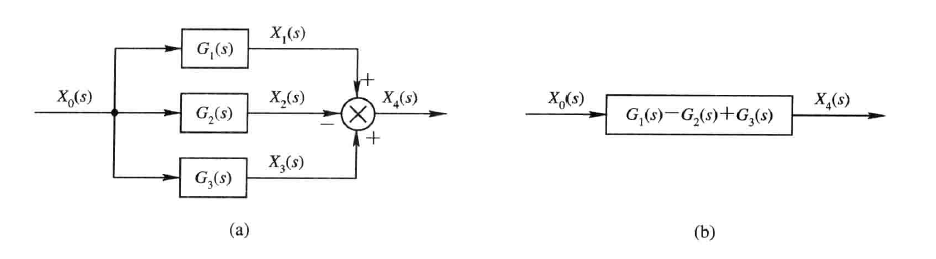
\includegraphics[width=8cm]{photos/并联简化.png}
\end{figure}

反馈回路的简化:
\begin{figure}[H]
    \centering
    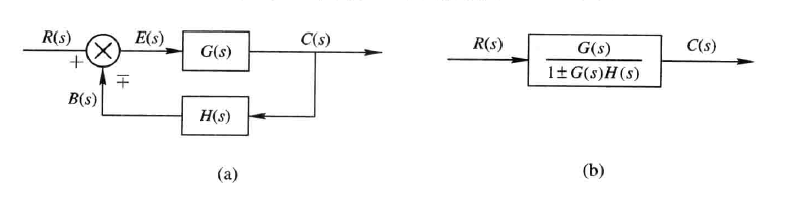
\includegraphics[width=8cm]{photos/反馈回路简化.png}
\end{figure}
\[
    G(s)=\frac{C(s)}{R(s)} = \frac{G(s)}{1\pm G(s)H(s)}
\]

相加点的前后移动:乘法分配律
\begin{figure}[H]
    \centering
    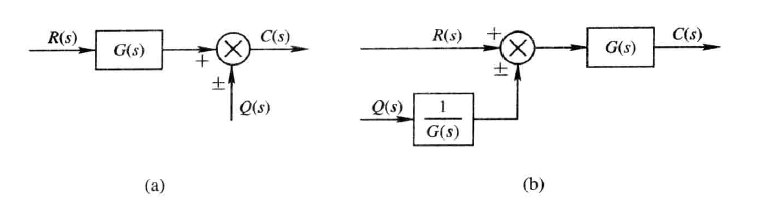
\includegraphics[width=8cm]{photos/相加点前移.png}
\end{figure}
\[
    C(s)=R(s)G(s)\pm Q(s)=[R(s)\pm \frac{Q(s)}{G(s)}]G(s)
\]
\begin{figure}[H]
    \centering
    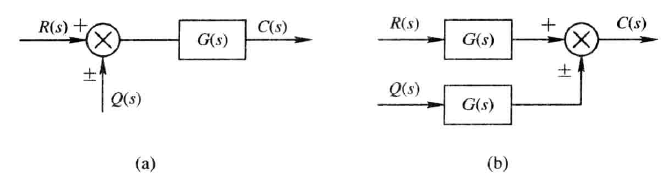
\includegraphics[width=8cm]{photos/相加点后移.png}
\end{figure}
\[
    C(s)=[R(s)\pm Q(s)]G(s)=R(s)G(s)\pm Q(s)G(s)
\]

分支点的移动类似.不多赘述

对于一个较复杂的系统,可以通过上述方法将其化简为一个简单的系统,
化简时关键在于同类点移动到同类点,不能跨越不同类点移动

\subsection{信号流图}
类比数据结构中的有向图,信号流图由节点和支路构成.

节点:表示系统中的变量或信号,例如输入信号、输出信号或中间变量

支路:表示信号的传递路径,箭头的方向指示信号的流动方向.
每条边上可能会标有增益或系统的传递函数,表示信号在传递过程中的变换.

\subsubsection{若干术语}

\textbf{输入节点(源)}:仅具有输出支路的节点.

\textbf{输出节点(阱)}:仅具有输入支路的节点.有时信号流图中没有一个节点是仅具有输入支
路的,我们只要定义信号流图中任一变量为输出变量,然后从该节点变量引出一条增益为
1的支路,即可形成一输出节点.

\textbf{混合节点}:既有输入支路又有输出支路的节点.

\textbf{通道}:支路箭头方向而穿过各相连支路的途径.如果通道与任一节点相交不多于一
次,就叫开通道.如果通道的终点就是起点,并且与任何其他节点相交不多于一次,就称
作闭通道.

\textbf{前向通道}:从输入节点到输出节点,通过的节点不多于一次的通道.

\textbf{前向通道增益}:向通道上各支路增益之乘积,用$P_k$表示.

\textbf{回路}:点和终点在同一节点,并与其它节点相遇仅一次的通路,也就是闭通道.

\textbf{回路增益}:回路中所有支路的乘积,用$L_a$表示.

\textbf{不接触回路}:回路之间没有公共节点时,这种回路叫做不接触回路.

\subsubsection{信号流图的性质}
(1)信号流图适用于线性系统.

(2)支路表示一个信号对另一个信号的函数关系,信号只能沿支路上的箭头方向传递.

(3)在节点上可以把所有输入支路的信号叠加,并把相加后的信号送到所有的输出支路.

(4)具有输入和输出支路的混合节点,通过增加一个具有单位增益的支路可以把它作为输出节点来处理.

(5)对于一个给定的系统,信号流图不是唯一的.由于描述同一个系统的方程可以表示为不同的形式,因此可以画出不同的信号流程图.

\subsubsection{梅森公式}

ppt和课本的梅森公式不将人话,这里用线性代数的语言描述,笔者尽可能的讲人话

考虑一个具有$n$个节点的信号流图.
设$x_i$​表示节点$i$的信号,$a_{ij}$​表示从节点$j$到节点$i$的支路增益,$u$表示输入信号,$y$表示输出信号.
每个节点的信号可以表示为所有指向该节点的信号之和,加上来自输入信号的直接贡献:
\[
    x_i = \sum_{j=1}^{n}a_{ij}x_j + b_iu
\]
其中,$b_i$是从输入节点到节点$i$的直接增益.

对于输出节点$y$,它可以是某个节点$k$的信号,或者节点信号的线性组合:
\[
    y = \sum_{j=1}^{n}c_jx_j
\]
其中,$c_j$是从节点$j$到输出的增益

将上述方程写成矩阵形式.

定义:
$\bf{x}=\begin{bmatrix}
    x_1\\
    x_2\\
    \vdots\\
    x_n
\end{bmatrix}$,
$\bf{A}=\begin{bmatrix}
    a_{11} & a_{12} & \cdots & a_{1n}\\
    a_{21} & a_{22} & \cdots & a_{2n}\\
    \vdots & \vdots & \ddots & \vdots\\
    a_{n1} & a_{n2} & \cdots & a_{nn}
\end{bmatrix}$,
$\bf{b}=\begin{bmatrix}
    b_1\\
    b_2\\
    \vdots\\
    b_n
\end{bmatrix}$,
$\bf{c}=\begin{bmatrix}
    c_1\\
    c_2\\
    \vdots\\
    c_n
\end{bmatrix}$.
则有$\bf{x}=\bf{Ax}+\bf{bu}$,$\bf{y}=\bf{c^Tx}$.

可以得到
\[
    \bf{x}=(\bf{E}-\bf{A})^{-1}\bf{bu}
\]

所以
\[
    \bf{y}=\bf{c^T}(\bf{E}-\bf{A})^{-1}\bf{bu}
\]

所以
\[
    \text{梅森公式:}\bf{T}=\bf{c^T}(\bf{E}-\bf{A})^{-1}\bf{b}
\]

$(\bf{E}-\bf{A})^{-1}$可以用下列公式计算
\[
    (\bf{E}-\bf{A})^{-1} = \frac{(\bf{E}-\bf{A})^*}{det(\bf{E}-\bf{A})}
\]

以上是梅森公式如何计算,下面是梅森公式的作用

用梅逊公式可以直接求信号流图从输入节点到输出节点的增益,可以用来求传递函数.

\section{线性系统的时域分析}
\subsection{典型输入信号}
\subsubsection{阶跃函数}
\[
    r(t)=\begin{cases}
        R\cdot 1(t),&t\geqslant 0\\
        0,& t<0
    \end{cases}
\]
当$R=1$时称为单位阶跃函数

\subsubsection{斜坡函数}
斜坡函数又称速度函数
\[
    r(t)=\begin{cases}
        Rt,&t\geqslant 0\\
        0,&t < 0
    \end{cases}
\]
当$R=1$时,称为单位斜坡函数

\subsubsection{加速度函数}
\[
    r(t)=\begin{cases}
        \frac{Rt^2}{2},&t\geqslant 0\\
        0,&t < 0
    \end{cases}
\]
当$R=1$时,称为单位加速度函数

\subsubsection{脉冲函数}
\[
    r(t)=\begin{cases}
        \frac{1}{h},&0<t<h\\
        0,&t\leqslant 0,t\geqslant h
    \end{cases}
\]
称$h$为脉冲宽度,脉冲面积为$1$.若取极限$\lim_{h\to 0}r(t)$,有
\[
    \delta(t)=\lim_{h\to 0}r(t)=\begin{cases}
        \infty,&t=0\\
        0,&t\neq 0
    \end{cases}
\]
以及
\[
    \int_{-\infty}^{+\infty}\delta(t)dt=1
\]
称此函数为理想脉冲函数

\subsubsection{正弦函数}
\[
    r(t)=A\sin (\omega t)
\]
$A$为振幅,$\omega$为角频率

\subsection{动态和稳态}
以下是一个系统的输出$c(t)$的变化
\begin{figure}[H]
    \centering
    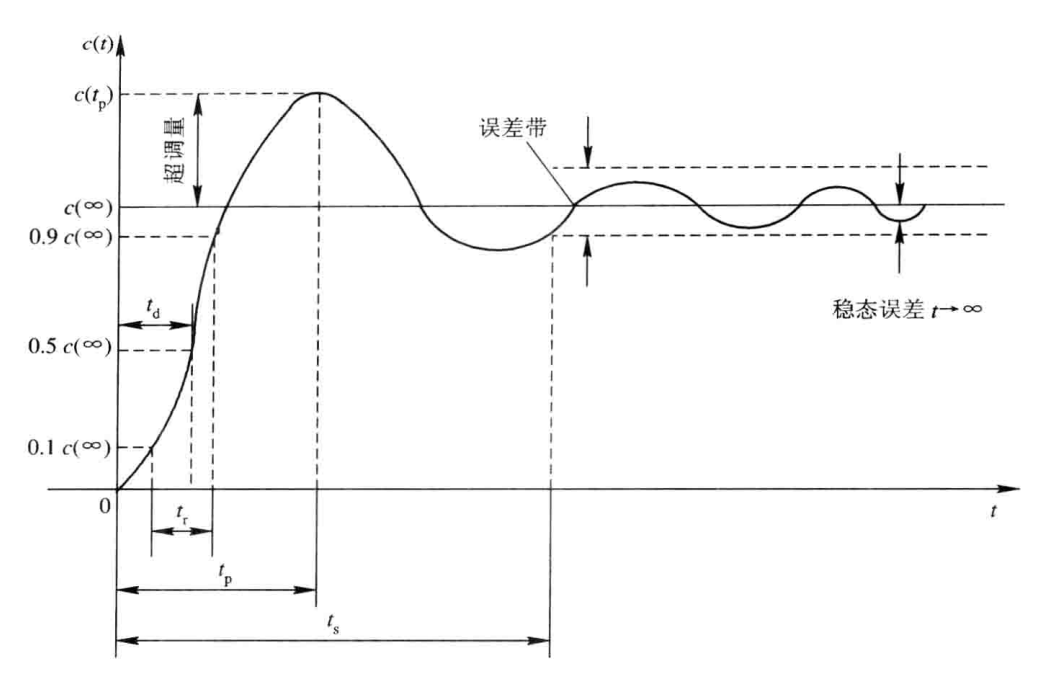
\includegraphics[width=8cm]{photos/系统动态性能指标.png}
\end{figure}

可以看到大体可以分为两段:前一段不断变化,起伏较大;后一段起伏较小,大体在某一值附近

前一段我们称之为动态过程;后一段称之为稳态过程

我们需要描述系统的性能,就有一些指标描述,我们分为动态性能与稳态性能描述

\subsubsection{动态性能}
动态性能指标通常有以下几种(图中有标注):

延迟时间$t_d$:指响应曲线第一次达到稳态值的一半所需的时间.

上升时间$t_{\tau}$:若阶跃响应不超过稳态值,上升时间指响应曲线从稳态值的$10\%$上升到$90\%$所需的时间;
对于有振荡的系统,上升时间定义为响应从零第一次上升到稳态值所需的时间.上升时间越短,响应速度越快.

峰值时间$t_p$:指阶跃响应曲线超过稳态值,到达第一个峰值所需要的时间.

调节时间$t_s$:在响应曲线的稳态线上,用稳态值的百分数(通常取$5\%$或$2\%$)作一个允许误差范围,响应曲线达到并永远保持在这一允许误差范围内所需的时间.

最大超调量$\sigma_p$:设阶跃响应的最大值为$c(t_p)$,则最大超调量可由下式确定:
\[
    \sigma_p = \frac{c(t_p)-c(\infty)}{c(\infty)} \times 100 \%
\]

振荡次数$N$:在$0\leqslant t\leqslant t_s$内,阶跃响应曲线穿越稳态值$c(\infty)$次数的一半称为振荡次数.


\end{document}